% Condensed author version. Preserves all results, labels, and figure input.
% Uses the existing theorem/lemma/corollary/proof environments.

\subsection{A Work-Sensitive Finite-Field Bound}
\label{ext:sec-profile}

Retain $n\ge r\ge2$, invertible $B$, and conditionally independent uniform
$U,V\in\mathbb F_q^{n\times r}$. Complete pre-input history fixes the
program and gate allocation, including arbitrary paid state; the complete
candidate precedes the checking vectors.

\begin{lemma}[Output-span agreement]
\label{ext:lem-output-span}
For $0\le s\le r$, define
\begin{equation}
\rho_s=q^{-nr}\prod_{i=0}^{s-1}
       \frac{(q^n-q^i)(q^r-q^i)}{q^s-q^i},
\label{ext:eq-rank-probability}
\end{equation}
with empty product one, and put
\begin{equation}
\mu_{n,r,q}(w)=\sum_{s=0}^{r}\rho_s q^{-(ns-w)_+},
\qquad (x)_+=\max\{x,0\}.
\label{ext:eq-mu}
\end{equation}
For every reachable pre-input history $\mathcal H^-$ and admitted $w$-gate program $F$,
\begin{equation}
\Pr[F(U,V)=UV^\top B\mid\mathcal H^-]\le\mu_{n,r,q}(w),
\label{ext:eq-span-agreement}
\end{equation}
with equality when $w=0$.
\end{lemma}

\begin{proof}
The outputs of $F=\sum_{a=1}^{w}Z_aL_a(U)R_a(V)$ belong to the fixed space
$Z=\operatorname{span}\{Z_1,\ldots,Z_w\}$, of dimension at most $w$.
Given rank-$s$ $U$, the independent uniform matrix $Y=V^\top B$ makes $UY$
uniform on its $ns$-dimensional image $\mathcal L_U$. Thus
\begin{equation}
\begin{aligned}
\Pr[F=UY\mid U,\mathcal H^-]
&\le\Pr[UY\in Z\mid U,\mathcal H^-]\\
&=q^{\dim(Z\cap\mathcal L_U)-ns}
 \le q^{-(ns-w)_+}.
\end{aligned}
\label{ext:eq-span-intersection}
\end{equation}
Counting full-rank $n\times s$ and $s\times r$ factorizations and dividing
by their $|\mathrm{GL}_s(\mathbb F_q)|$ multiplicity gives the rank
probabilities~\eqref{ext:eq-rank-probability}~\cite{LaksovThorup1994}.
Averaging proves the claim, including zero and rank-deficient inputs.
At $w=0$, $F=0$, and conditional agreement has probability $q^{-ns}$.
\end{proof}

\paragraph{Comparison with bilinear agreement bounds}
\label{sec:profile-comparison}
Cohen and Moshkovitz establish
$\operatorname{AR}(D)\ge(1-\log_q2)\operatorname{GR}(D)$ and
$\operatorname{AR}(D)=-\log_q\Pr[D=0]$ for uniform bilinear inputs
\cite[Proposition~4.1 and Fact~4.5]{cohen2022structure}. Rectangular multiplication has geometric
rank $g=nr-\lfloor r^2/4\rfloor$~\cite{kopparty2023geometric}
and slice rank $nr$ even over the algebraic closure, by its
semistability~\cite[Example~24 and Lemma~23]{christandl2023weighted}.\footnote{If a slice decomposition uses dimensions $a_i$ in modes of
dimensions $m_i$ with $\sum_i a_i<\min_i m_i$, assign weights
$1-a_i/m_i$ to its subspaces and $-a_i/m_i$ to their complements.
After clearing denominators, each factor has total weight zero, while
every supported tensor term has positive weight
$\ge1-\sum_i a_i/m_i$. This contradicts semistability. The reverse
bound follows by slicing a smallest mode.}
For $D=T-F$, take slice rank over the algebraic closure.
Subadditivity gives $\operatorname{SR}(D)\ge nr-w$ and
$\operatorname{GR}(D)\ge g-w$. Cohen--Moshkovitz's proof gives
$\operatorname{SR}(D)\le2\operatorname{GR}(D)$ over that closure
\cite[proof of Theorem~3.1]{cohen2022structure}; no descent is needed.
Since geometric rank is integral, their finite-field analytic-rank
inequality yields
\begin{equation}\label{eq:cm-field-comparator}
 \Pr[F=T]\le (2/q)^{\max\{\lceil(nr-w)/2\rceil,\,g-w,\,0\}},\quad q>2.
\end{equation}
An elementary comparison also uses the exact zero probability:
a uniform-input bilinear map's largest output atom occurs at zero
\cite[proof of Proposition~5.1]{cohen2022structure}. The fixed range of
$F$ has at most $q^w$ points, giving
$B_{\rm range}(w)=\min\{1,q^w\mu(0)\}$. Concavity of $z\mapsto\min\{1,z\}$ gives
\begin{equation}\label{eq:profile-vs-range}
 \mu(w)=\E_s\min\{1,q^{w-ns}\}\le B_{\rm range}(w).
\end{equation}
This is strict for every integer $0<w<nr$: the positive rank-zero
mass makes $\mu(w)<q^w\mu(0)$, and positive full-rank mass makes
$\mu(w)<1$. At $w=0$ the two range bounds coincide exactly.
At $n=16,r=4,q=17,w=56$, $\mu(w)=1.434\times10^{-10}$,
$B_{\rm range}(w)=1.426\times10^{-5}$, and
\eqref{eq:cm-field-comparator} gives $1.916\times10^{-4}$.
The rank-conditioned argument also covers $q=2$, where the geometric
comparison's coefficient vanishes. Below a certified tensor-rank
threshold, all three bounds can also use the common cap $2/q-1/q^2$;
checking then applies $p\mapsto p+(1-p)q^{-t}$.


Choose a certified integer lower bound $1\le R_0\le R=\mathcal R_q(n,r,n)$;
Lemma~\ref{lem:fresh-tensor} permits $R_0=n^2$, without asserting equality
to $R$. Write $\mu(w)=\mu_{n,r,q}(w)$, $\vartheta=2/q-1/q^2$, and define
\begin{equation}
\overline p(w)=
\begin{cases}
\min\{\vartheta,\mu(w)\},&0\le w<R_0,\\
1,&w\ge R_0,
\end{cases}
\label{ext:eq-pbar}
\end{equation}
and, for predetermined $t_j$,
\begin{equation}
\mathsf{Acc}_j(w)=\overline p(w)+(1-\overline p(w))q^{-t_j}.
\label{ext:eq-work-acceptance}
\end{equation}

\begin{corollary}[A conditional acceptance profile]
\label{ext:cor-work-acceptance}
At every reachable pre-input history, exact-increment and acceptance
probabilities are at most $\overline p(w)$ and $\mathsf{Acc}_j(w)$,
respectively, even with an incorrect previous reference.
\end{corollary}

\begin{proof}
For $w<R_0\le R$, a nonzero bilinear coordinate of the discrepancy
vanishes with probability at most $\vartheta$ by
Theorem~\ref{thm:fresh-one}. Combining Lemma~\ref{ext:lem-output-span}
gives~\eqref{ext:eq-pbar}; for $w\ge R_0$ the bound is trivial.
The candidate and checker use the same old reference, leaving discrepancy
$D=F(U,V)-UV^\top B$ regardless of prior errors. A fixed nonzero $D$
passes all checks with probability $q^{-t_j\operatorname{rank}D}\le q^{-t_j}$.
Conditioning on $D=0$ proves~\eqref{ext:eq-work-acceptance}.
\end{proof}

Increment and complete-product agreement coincide only with a genuine
reference. Acceptance can be strictly smaller even at $w=0$ when the
nonzero discrepancy has rank above one. Transforms, state access,
materialization, and checking retain their separate costs.

\subsection{Adaptive Rounds Under a Pathwise Work Budget}
\label{ext:sec-profile-dp}

\begin{theorem}[Aggregate work-profile bound]
\label{ext:thm-profile-dp}
Consider $k$ prescribed rounds under the preceding conditional freshness
assumptions, predetermined $t_1,\ldots,t_k$, and $\sum_jw_j\le W$ on every
path. Put $\overline W=\lfloor W\rfloor$ and $G_{k+1}(z)=1$ for integer
$z\ge0$. Define backwards
\begin{equation}
G_j(z)=\max_{\substack{w\in\mathbb Z_{\ge0}\\w\le z}}
       \mathsf{Acc}_j(w)G_{j+1}(z-w).
\label{ext:eq-profile-dp}
\end{equation}
Then
\begin{equation}
\begin{aligned}
&\Pr[\text{all $k$ rounds execute and accept}]\le G_1(\overline W)\\
&\hspace{5mm}=
 \max_{\substack{\mathbf w\in\mathbb Z_{\ge0}^{k}\\
                  \sum_jw_j\le\overline W}}
       \prod_{j=1}^{k}\mathsf{Acc}_j(w_j).
\end{aligned}
\label{ext:eq-profile-product}
\end{equation}
Replacing $\mathsf{Acc}_j(w)$ by $\overline p(w)$ bounds the event that
all $k$ rounds execute with exact increments.
\end{theorem}

\begin{proof}
At a pre-input history with remaining budget $z$ and selected allocation
$w$, Corollary~\ref{ext:cor-work-acceptance} bounds acceptance by
$\mathsf{Acc}_j(w)$. Every accepted continuation has budget at most $z-w$;
backward induction bounds its success by $G_{j+1}(z-w)$ uniformly over
complete histories, including incorrect references. Maximizing over $w$
proves~\eqref{ext:eq-profile-dp}; randomized choices are mixtures.
Aborts and rejections fail the event. Expanding the recurrence proves
\eqref{ext:eq-profile-product}; replacing acceptance by exactness proves
the final statement. Cross-round independence is unnecessary.
\end{proof}

\paragraph{Finite actions and the threshold comparison}
Since $\mu(w)=1$ for $w\ge nr$, the actions reduce to
\begin{equation}
\mathcal A=\{0,\ldots,\min(nr,R_0-1)\}\cup\{R_0\},
\label{ext:eq-dp-actions}
\end{equation}
intersected with the remaining budget. If $nr<R_0$, retain $nr$ as the
least-cost representative of the $\overline p(w)=\vartheta$ plateau
through $R_0-1$; $R_0$ represents all larger actions. These replacements
preserve profile values at no greater cost. The bound is one for
$\overline W\ge kR_0$.
For the default $R_0=n^2$, improvement over the threshold profile
requires $w<nr$, or normalized work $w/R_0<r/n$.

With acceptance coefficients precomputed and
$M=|\mathcal A|\le\min(nr,R_0-1)+2$, value computation takes
$O(k(\overline W+1)M)$ arithmetic operations/comparisons and
$O(\overline W+1)$ auxiliary dynamic-programming (DP) storage. Recovering an allocation stores
one maximizing action per state, requiring $O(k(\overline W+1))$
additional entries. These are arithmetic/comparison-model counts.
Replacing $\overline p(w)$ below $R_0$ by $\vartheta$ recovers the threshold
bound: free below-threshold rounds and at most
$\min\{k,\lfloor W/R_0\rfloor\}$ threshold-reaching rounds.
The profile strengthens it pointwise.

\paragraph{An analytical example}
For $n=4,r=2,q=2,k=4,W=8,t_j=1,R_0=16$, the $256$ matrices $U$
have rank counts $(1,45,210)$. Hence
\begin{equation}
\mu(w)=\frac{1+45\,2^{-(4-w)_+}+210\,2^{-(8-w)_+}}{256}.
\label{ext:eq-profile-example}
\end{equation}
Here $\mu(0)=593/32768$, $\mu(7)=151/256<\vartheta=3/4$, and
$\mu(8)=1$, so action $8$ is essential. A maximizing allocation is
$(8,0,0,0)$ up to permutation, giving
\begin{equation}
\begin{aligned}
G_1(8)&=\frac78\left(\frac{33361}{65536}\right)^3\approx0.115421,\\
\text{threshold bound}&=\left(\frac78\right)^4\approx0.586182.
\end{aligned}
\label{ext:eq-profile-example-result}
\end{equation}
Indeed, $\log\mathsf{Acc}(w)=\log(A+B2^w)$ is convex on $[0,4]$
for positive $A,B$, concentrating work at the endpoints. At most one
allocation exceeds four; comparing $(4,4),(5,3),(6,2),(7,1),(8,0)$
with the other two allocations zero establishes the maximum.

\begin{figure*}[t]
  \centering
  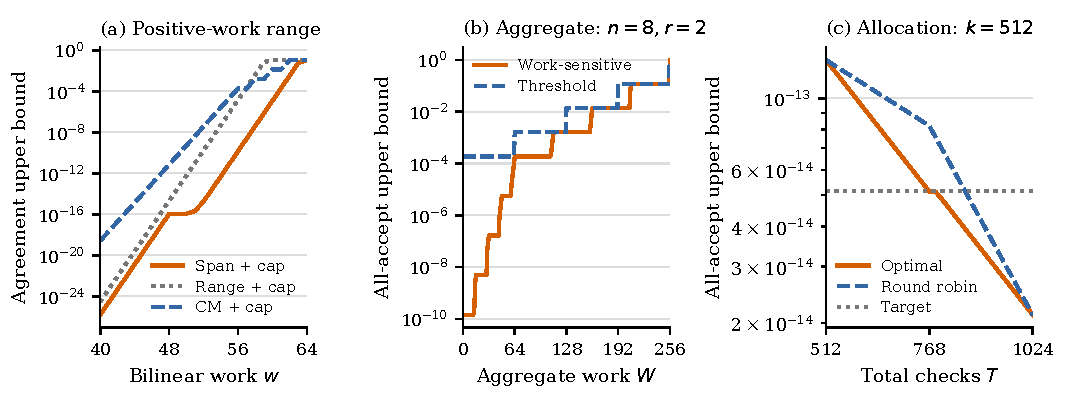
\includegraphics[width=\textwidth]{figures/theory_bounds_v4.pdf}
  \caption{Analytical agreement, all-accept bounds, and optimal checking allocations under the stated work-budget hypotheses.}
  \label{fig:theory-bounds}
\end{figure*}

Figure~\ref{fig:theory-bounds} compares these analytical bounds and the
checking allocations below.

\subsection{Single-Round Sharpness}
\label{ext:sec-sharpness}

Karppa and Kaski's six-product Strassen--Winograd variant omits an output
monomial~\cite[Sec.~1.1]{KarppaKaski2019}. A witness from Strassen's
identity~\cite{strassen} attains our one-round bound.

\begin{theorem}[Sharpness of the one-round threshold]
\label{ext:thm-sharpness}
For every finite field $\mathbb F_q$, $t\ge1$, $n=r=2$, and invertible
$B$, an admitted six-gate program has exact-increment probability
$\vartheta=2/q-1/q^2$ and acceptance probability exactly
$\vartheta+(1-\vartheta)q^{-t}$. Its six gates are fewer than the exact
threshold $\mathcal R_q(2,2,2)=7$.
\end{theorem}

\begin{proof}
Write $U=\left[\begin{smallmatrix}a&b\\c&d\end{smallmatrix}\right]$,
$Y=V^\top B=\left[\begin{smallmatrix}e&f\\g&h\end{smallmatrix}\right]$.
Compute
\[
\begin{aligned}
P_1&=(a+d)(e+h),&P_2&=(c+d)e,\\
P_3&=a(f-h),&P_4&=d(g-e),\\
P_5&=(a+b)h,&P_7&=(b-d)(g+h),
\end{aligned}
\]
and return
\[
F_6=\begin{bmatrix}
P_1+P_4-P_5+P_7&P_3+P_5\\
P_2+P_4&P_1-P_2+P_3
\end{bmatrix}.
\]
The seven-product identity gives
\begin{equation}
F_6-UY=-E_{22}(c-a)(e+f).
\label{ext:eq-missing-product}
\end{equation}
The omitted product is never computed. Its two linear forms are independent
uniform field elements, including in characteristic two, so their product
vanishes with probability $1-(1-1/q)^2=\vartheta$. Otherwise the discrepancy
has rank one and passes $t$ independent checks with probability exactly
$q^{-t}$. The invertible input change preserves the six-gate representation;
$\mathcal R_q(2,2,2)=7$ over every field~\cite{BlaserChristandlZuiddam2017}.
\end{proof}

This existing missing-term technique proves single-round sharpness;
each witness consumes six gates, with no aggregate tightness claim.

\subsection{Selecting and Distributing Checking Work}
\label{ext:sec-checking-design}

Checking counts are predetermined and equally costly; programs may still
adapt to prior history.

\begin{corollary}[A closed-form checking rule]
\label{ext:cor-target}
Put $b=\min\{k,\lfloor W/R_0\rfloor\}$, $d=k-b>0$, and
$\alpha(t)=\vartheta+(1-\vartheta)q^{-t}$.
For $\delta\in(0,1)$, the uniform threshold certificate
$\alpha(t)^d\le\delta$ holds exactly when
\[
d\ge\left\lceil\frac{\log\delta}{\log\alpha(t)}\right\rceil.
\]
For fixed $d$, a finite $t$ exists exactly when $\delta>\vartheta^d$;
the smallest permitted integer is
\begin{equation}
t_{\min}=\max\left\{1,
\left\lceil\log_q\frac{1-\vartheta}{\delta^{1/d}-\vartheta}\right\rceil
\right\}.
\label{ext:eq-target-t}
\end{equation}
\end{corollary}

\begin{proof}
The equivalent inequality
$q^{-t}\le(\delta^{1/d}-\vartheta)/(1-\vartheta)$ requires a positive
right side for finite $t$. Taking logarithms gives both expressions.
\end{proof}

For $d=0$ the certificate is one. Verify numerical ceilings in the original
inequality. The floor $\vartheta^d$ concerns this threshold certificate;
use~\eqref{ext:eq-profile-dp} for the stronger profile.

\begin{theorem}[Balanced checking for identical rounds]
\label{ext:thm-balanced}
Assume identical $n,r,q,\overline p$ and equal checking costs. Among integer
$t_j\ge1$ with $\sum_jt_j=T\ge k$, a balanced allocation minimizes both
the threshold and work-profile certificates. Write $T=k\ell+s$,
$0\le s<k$. A minimizer has $k-s$ entries $\ell$ and $s$ entries $\ell+1$;
its threshold value, for $d=k-b$, is
\begin{equation}
\alpha(\ell)^{\min\{d,k-s\}}\,
\alpha(\ell+1)^{\max\{0,d-k+s\}}.
\label{ext:eq-balanced-threshold}
\end{equation}
Its work-profile value is given by~\eqref{ext:eq-profile-dp}.
\end{theorem}

\begin{proof}
For $c\in[0,1]$, $f_c(x)=\log[c+(1-c)q^{-x}]$ is convex. Thus
\[
H(\mathbf t)=
\max_{\substack{\mathbf w\in\mathbb Z_{\ge0}^k\\
                \sum_jw_j\le\lfloor W\rfloor}}
\sum_j f_{\overline p(w_j)}(t_j)
\]
is convex; identical profiles and a permutation-invariant budget make it
symmetric. The log threshold certificate, a maximum of sums of $d$
functions $f_\vartheta(t_j)$, has the same properties.
For integers $u-v\ge2$, replacing $(u,v)$ by $(u-1,v+1)$ averages the
original pair with its swap, with swap weight $1/(u-v)$.
Convexity and symmetry cannot increase either objective. Iteration reaches
the stated balanced allocation. Its $d$ largest $\alpha(t_j)$ contain
$\min\{d,k-s\}$ copies of $\alpha(\ell)$, proving the formula.
\end{proof}

If $s\le b$, the exceptional set contains all strengthened rounds and the
threshold value remains $\alpha(\ell)^d$; the profile still uses its recurrence.

\subsection{Heterogeneous Checking Allocation}
\label{ext:sec-heterogeneous}

For the predetermined history-uniform parameters of
Theorem~\ref{thm:fresh-stateful}, put
$\vartheta_j=1-\lambda_{U,j}\lambda_{V,j}$ and
\[
\alpha_j(t)=\vartheta_j+(1-\vartheta_j)q^{-t},\qquad
c_j(t)=-\log\alpha_j(t).
\]
For a valid bound $b<k$ on threshold-reaching rounds and $d=k-b$, optimize
\begin{equation}
\Psi(\mathbf t)=\max_{\substack{E\subseteq[k]\\|E|\le b}}
                     \prod_{j\notin E}\alpha_j(t_j)
\label{ext:eq-hetero-objective}
\end{equation}
over integer $t_j\ge1$, $\sum_jt_j=T\ge k$.
We specialize ordered-sum thresholds~\cite{OgryczakTamir2003} and greedy
concave resource allocation~\cite{FedergruenGroenevelt1986}.

\begin{theorem}[An exact heterogeneous checking allocation]
\label{ext:thm-heterogeneous}
Under equal checking costs and the preceding parameters, form
\[
\mathcal C=\{c_j(u):1\le j\le k,\ 1\le u\le T-k+1\}.
\]
For each $\tau\in\mathcal C$, start with $t_j=1$ and repeatedly allocate
the remaining $T-k$ checks to a round maximizing
\begin{equation}
\Delta_j=\min\{c_j(t_j+1),\tau\}-\min\{c_j(t_j),\tau\},
\label{ext:eq-hetero-gain}
\end{equation}
breaking ties by fixed index. Select the candidate and threshold maximizing
\begin{equation}
\sum_j\min\{c_j(t_j),\tau\}-b\tau.
\label{ext:eq-hetero-score}
\end{equation}
The selected allocation globally minimizes $\Psi$ at budget $T$.
\end{theorem}

\begin{proof}
Since $0<\alpha_j\le1$, $-\log\Psi$ is the sum of the $d$ smallest
$c_j(t_j)$. In nondecreasing order $c_{(i)}$, the ordered-sum identity is
\begin{equation}
\sum_{i=1}^{d}c_{(i)}=
\max_{\tau\ge0}\left\{\sum_j\min(c_j,\tau)-b\tau\right\}.
\label{ext:eq-ordered-sum}
\end{equation}
Its slope is the number of entries above $\tau$ minus $b$; hence
$\tau=c_{(d)}$ maximizes it, including ties and $b=0$.
For fixed $\tau$, $\min\{c_j(t),\tau\}$ is nondecreasing and concave.
Its discrete gains are nonnegative and nonincreasing. Each feasible
allocation takes a prefix of every gain sequence. Taking the largest
available gain preserves these prefixes and selects the largest remaining
gains, proving fixed-threshold greedy optimality.
Every feasible $t_j\le T-k+1$, so an optimal allocation's threshold
$c_{(d)}$ belongs to $\mathcal C$. Interchanging the two maximizations and
enumerating that set therefore attains the global optimum.
\end{proof}

Put $S=T-k$. At most $k(S+1)$ thresholds each require $S$ allocations.
A heap uses $O(k(S+1)(k+S\log k))$ reward comparisons in the
exact-comparison model, giving pseudo-polynomial complexity.
Parameters must remain uniform over all reachable histories, including
incorrect acceptances. Optimality concerns~\eqref{ext:eq-hetero-objective},
not the heterogeneous work-profile minimax objective or actual attack probability.


\paragraph{Local descent and integrity requirements}
Directly maximizing the one-step decrease of $\Psi$ need not be globally
optimal. For $k=3,b=2,q=17,\vartheta_j=15/16,T=6$, all available gains
are zero along the fixed-smallest-index greedy path from $(1,1,1)$.
It returns $(4,1,1)$ with $\Psi=16/17$, whereas $(2,2,2)$ gives
$271/289<16/17$.

Conditional checking soundness and a union bound limit the probability
of any incorrect accepted increment by $I(\mathbf t)=\sum_jq^{-t_j}$,
without independence across rounds. For $0<\vartheta_j\le1$, define
\[
 f_\infty=\max_{\substack{E\subseteq[k]\\|E|\le b}}
               \prod_{j\notin E}\vartheta_j,
 \qquad \kappa=\max_j\frac{1-\vartheta_j}{\vartheta_j}.
\]
Then
\begin{equation}\label{eq:integrity-work-link}
 f_\infty\le\Psi(\mathbf t)
       \le f_\infty\exp\!\bigl(\kappa I(\mathbf t)\bigr).
\end{equation}
Indeed, $\alpha_j(t)=\vartheta_j[1+(1-\vartheta_j)q^{-t}/\vartheta_j]$;
apply $1+x\le e^x$ to each retained factor and maximize over $E$.

Theorem~\ref{ext:thm-heterogeneous} also holds with integer minima
$t_j\ge L\ge1$ and $T\ge kL$: start from $L$, allocate $T-kL$ checks, and enumerate
\[
 \mathcal C_L=\{c_j(u):j\in[k],\ u=L,\ldots,T-(k-1)L\}.
\]
The same threshold and decreasing-gain proof gives global optimality
among allocations obeying these minima.
For $0<\varepsilon<1$, choosing
$L=\max\{1,\lceil\log_q(k/\varepsilon)\rceil\}$ ensures
$I(\mathbf t)\le\varepsilon$; this common minimum is a sufficient
condition for a general integrity budget.
